\documentclass[aspectratio=169]{beamer}

\usepackage{tikz}
\usepackage{tikzducks,tikzlings}

\setbeamertemplate{background canvas}{
  \begin{tikzpicture}[remember picture,overlay]
    \node[anchor=south,inner sep=0pt] at (current page.south) {\includegraphics[width=\paperwidth]{Andaman_Sea_at_night,_Moonset,_Moonlight}};
    % credit for background image
    \node[white,text width=\paperwidth,font=\tiny,align=center] at ([yshift=0.25cm]current page.south) {Image by Vyacheslav Argenberg (\url{https://commons.wikimedia.org/wiki/File:Andaman_Sea_at_night,_Moonset,_Moonlight.jpg})};
  \end{tikzpicture}
}

\setbeamertemplate{navigation symbols}{}

% trick taken from https://topanswers.xyz/tex?q=1989
\tikzset{
    use page relative coordinates/.style={
        shift={(current page.south west)},
        x={(current page.south east)},
        y={(current page.north west)}
    }
}

\makeatletter
\newcommand*{\slideinframe}{\number\beamer@slideinframe}
\makeatother

\begin{document}

\def\steps{700}
\begin{frame}
  \begin{tikzpicture}[
      remember picture,
      overlay,
      use page relative coordinates,
    ]

    \begin{scope}
      \clip (0.6,0.35) rectangle (1,1);
      \node[anchor=south] at (0.8,0.25-0.3*\slideinframe/\steps) {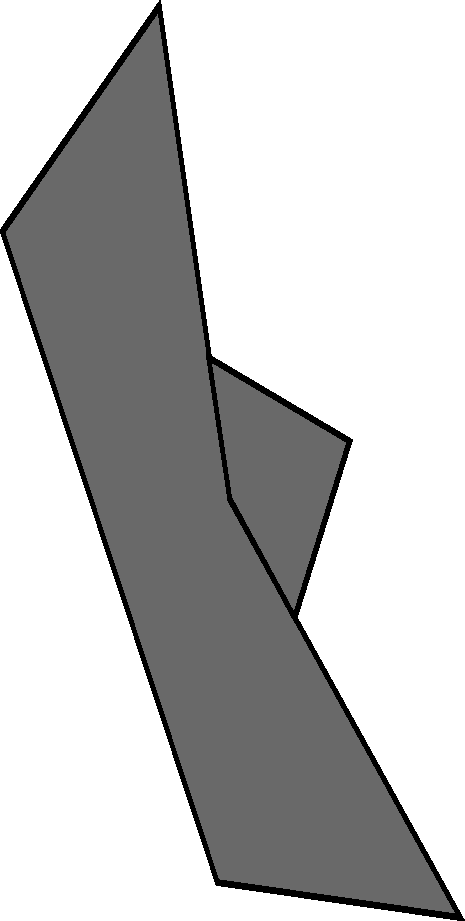
\includegraphics[width=1.5cm]{ship}};
    \end{scope}
    
    \node[rotate=3*sin(\slideinframe*3)] at (0.4,0.3) {
\includegraphics[width=7cm]{door}};

  \end{tikzpicture}
  \pause[\steps]
\end{frame}

\end{document}